\section{Methodology}

\subsection{Human Voice Detection Model}
This study focuses on developing a lightweight acoustic model capable of distinguishing between human and non-human sounds for search-and-rescue (SAR) robotics. The model is optimized for deployment on edge devices using TinyML frameworks. The training pipeline involves dataset preparation, feature extraction, data augmentation, and supervised learning.

\subsubsection{Dataset Collection and Labeling}
We utilized a subset of the publicly available CHiME-Home dataset~\cite{Foster2015chime}, which contains domestic environmental audio recordings annotated with sound event labels. Audio segments featuring human vocal activity such as speech, calling, or shouting were manually extracted and labeled as “human,” while other segments (e.g., background noise, domestic appliances, animals) were labeled as “non-human.” The dataset was further balanced and curated to ensure consistent segment lengths of three seconds at a sampling rate of 16\,kHz.

\subsubsection{Spectrogram Feature Extraction}
To convert the audio signals into a format suitable for convolutional neural networks (CNNs), we applied mel-spectrogram transformation. Each audio clip was transformed into a 64-bin mel-spectrogram using a short-time Fourier transform (STFT) with parameters tuned for low-latency environments. The resulting spectrograms were normalized to a \([0, 1]\) range after applying logarithmic scaling and clipping to \([-80, 0]\) dB.

The mel-spectrogram extraction process can be summarized as follows:

\begin{verbatim}
for each audio file in dataset:
    load audio at 16kHz mono
    if audio is empty:
        skip file
    compute mel-spectrogram with 64 mel bands
    convert to decibel (log) scale
    clip values to [-80, 0] dB
    normalize to [0, 1] range
    resize to 64x64 using interpolation
    save as .npy file
\end{verbatim}

\subsubsection{Data Augmentation}
To improve generalization and robustness in noisy or reverberant environments, two augmentation strategies were employed:

\begin{itemize}
  \item \textbf{Additive Gaussian Noise:} Small random noise was added to spectrograms to simulate environmental interference.
  \item \textbf{Time Masking:} Inspired by SpecAugment~\cite{Park2019specaugment}, random temporal sections of spectrograms were zeroed out to simulate partial occlusion of acoustic features.
\end{itemize}

Each original spectrogram generated two augmented variants, tripling the effective dataset size.

\subsubsection{Model Training and Evaluation}
The dataset was split using stratified sampling into training and testing subsets (80\% / 20\%). The model architecture consisted of a compact 2D convolutional neural network designed to fit within the memory constraints of embedded hardware. The input shape was fixed at $64 \times 64 \times 1$. The model was trained using binary cross-entropy loss and Adam optimizer, with early stopping and learning rate reduction callbacks to prevent overfitting.

The model architecture consisted of a series of convolutional and normalization layers, followed by pooling and fully connected layers. A detailed summary of the model is as follows:

\begin{itemize}
  \item \textbf{Input:} $64 \times 64 \times 1$ grayscale mel-spectrogram
  \item \textbf{Conv2D:} 32 filters, $3 \times 3$ kernel, ReLU activation
  \item \textbf{BatchNormalization}
  \item \textbf{Conv2D:} 32 filters, $3 \times 3$ kernel, ReLU activation
  \item \textbf{BatchNormalization}
  \item \textbf{MaxPooling2D:} $2 \times 2$
  \item \textbf{Conv2D:} 64 filters, $3 \times 3$ kernel, ReLU activation
  \item \textbf{BatchNormalization}
  \item \textbf{Conv2D:} 64 filters, $3 \times 3$ kernel, ReLU activation
  \item \textbf{BatchNormalization}
  \item \textbf{MaxPooling2D:} $2 \times 2$
  \item \textbf{Conv2D:} 128 filters, $3 \times 3$ kernel, ReLU activation
  \item \textbf{BatchNormalization}
  \item \textbf{Conv2D:} 128 filters, $3 \times 3$ kernel, ReLU activation
  \item \textbf{BatchNormalization}
  \item \textbf{GlobalAveragePooling2D}
  \item \textbf{Dense:} 128 units, ReLU activation
  \item \textbf{Dropout:} rate 0.5
  \item \textbf{Output:} Dense layer with 1 unit and sigmoid activation
\end{itemize}

The model was compiled with the Adam optimizer (learning rate = 0.0005) and binary cross-entropy loss. To address class imbalance, class weights were applied during training. Early stopping (patience = 10) and learning rate reduction on plateau (patience = 5, factor = 0.5) were employed to enhance convergence. The final model was trained over a maximum of 50 epochs with a batch size of 64.

Evaluation was performed on the held-out test set using standard classification metrics including accuracy, precision, recall, F1-score, and confusion matrix. The final model achieved a test accuracy of 97.79\%, demonstrating strong generalization performance in distinguishing human from non-human sounds.

\subsection{Weighted Centroid Localization}
We collected RSSI measurements in an indoor corridor (Labtek 1 Mekanika Tanah, ITB) using three fixed ESP32 beacons and one mobile ESP32 receiver. Measurements were taken at five known distances (1.60m, 2.40m, 3.20m, 4.00m, 4.80m) yielding a total of 1574 samples. Each sample consists of the RSSI value from a beacon at a given distance. These raw RSSI values were then preprocessed to support distance estimation: \begin{itemize}

\item {\bf Log-distance transform:} We converted the RSSI (in dBm) to an equivalent distance using the log-distance path-loss model. In practice, this means modeling $\text{RSSI}\approx -10n\log_{10}(d)+C$ (where $n$ is the path-loss exponent) to linearize the RSSI–distance relationship

\item {\bf Gaussian noise injection:} To improve robustness against channel variations, we added small zero-mean Gaussian noise to the RSSI samples during preprocessing. Prior work shows that training with artificial noise can yield more stable distance estimates.

\item {\bf Synthetic data augmentation:} We generated additional (synthetic) RSSI-distance pairs by interpolating between measured values so that the full RSSI range was covered uniformly. This ensures that the neural network sees examples spanning the entire operating spectrum of RSSI values.

\end{itemize} After preprocessing, we trained a separate neural network model for each beacon. Each model is an 8-layer fully connected (feedforward) neural network implemented in TensorFlow. The network takes the preprocessed RSSI as input and outputs a predicted distance. All hidden layers use ReLU activation and the final layer is linear. Inputs were standardized before training to improve convergence. This MLP approach is similar to prior RSSI‐localization work.

\begin{figure}[!b]
  \centering
  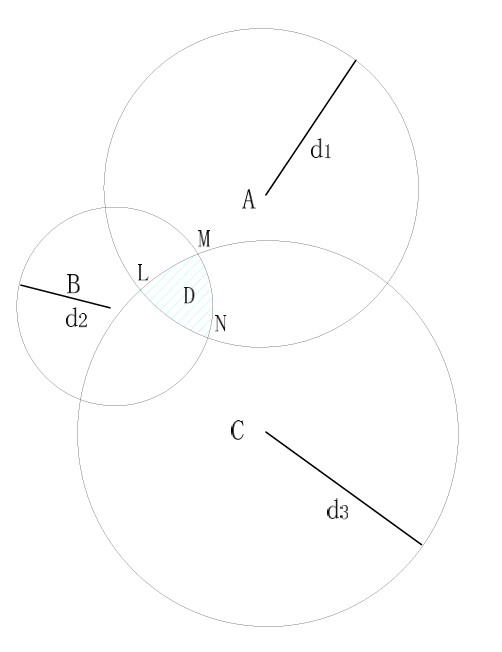
\includegraphics[width=0.5\linewidth]{img/fig2.jpg}
  \caption{Centroid positioning. D showing the possible positions of the robot, from beacon A, B, and C \cite{WSNCentroid}}
  \label{fig:centroid}
\end{figure}

\begin{figure}[!b]
  \centering
  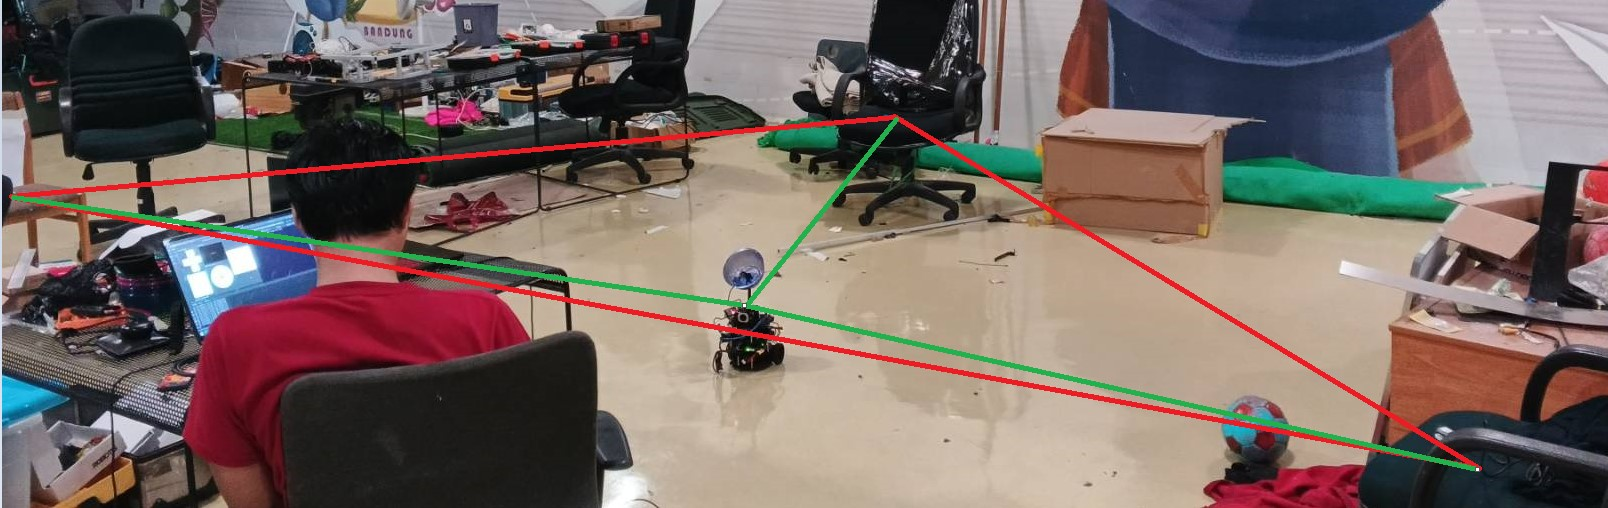
\includegraphics[width=0.75\linewidth]{img/rssi.jpg}
  \caption{Weighted Centroid Localization testing on different environment setup}
  \label{fig:environment}
\end{figure}

We trained each model on the 1574-sample dataset (combining all distances) and reserved a held-out set of 236 real (non-synthetic) measurements for testing. During training, we optimized with a standard gradient-based optimizer (e.g.\ Adam) until convergence. For localization, each beacon’s predicted distance defines a circle around that beacon with radius equal to the estimated distance. We then apply the triangle‐centroid method: the unknown tag is located at the centroid of the intersection region of the three circles (Fig.~\ref{fig:centroid}). As Zhang and Zhao \cite{WSNCentroid} describe, the algorithm uses RSSI to measure distances $d$, treats the beacon node as the center of a circle, the distance $d$ as the radius of each circle, and obtains the unknown node location by seeking the centroid of the three-circle intersection. 

In practice we compute the pairwise intersection points of the circles and take their centroid as the position estimate. To reduce bias from larger errors at greater distances, we apply a distance-based weighting: intersections involving shorter predicted distances are given higher weight when computing the centroid. This follows the idea of weighted centroid localization \cite{nagah2021enhanced}. The final estimated coordinates are thus a weighted centroid of the three-circle intersection, which yields a single $(x,y)$ position. All steps above—from data collection through model training and localization—were implemented in TensorFlow and evaluated using the held-out test set of 236 samples. Performance was reported as the error between the true and estimated positions in the lab.

To evaluate generalization, we also performed \emph{cross-environment testing}: after training exclusively in the Labtek 1 environment, we deployed the same models and localization pipeline in a different indoor space as shown in Fig.~\ref{fig:environment}. RSSI data were collected at the same five distances under this new setting, and localization accuracy was measured without any retraining. This assessment demonstrates the robustness of our distance regression and weighted triangle-centroid method to changes in multipath and clutter.

The ESP-32 positioning workflow can be expressed as follows:
\begin{lstlisting}
loop forever:
    beacons <- wifi_scan_beacons()
    foreach beacon in beacons:
        distances[beacon.ssid] <-
            model_predict_distance(beacon.rssi)
    beacons_position_relative <-
        get_beacons_relative_position(
            beacons_position_fixed,
            distances
        )

    send_uart(beacons_position_relative)
		
    wait for 1 second
\end{lstlisting}